\documentclass[preprint,12pt]{elsarticle}
\makeatletter
\def\ps@pprintTitle{%
 \let\@oddhead\@empty
 \let\@evenhead\@empty
 \def\@oddfoot{\centerline{\thepage}}%
 \let\@evenfoot\@oddfoot}
\makeatother


%% Use the option review to obtain double line spacing
%% \documentclass[preprint,review,12pt]{elsarticle}

%% Use the options 1p,twocolumn; 3p; 3p,twocolumn; 5p; or 5p,twocolumn
%% for a journal layout:
%% \documentclass[final,1p,times]{elsarticle}
%% \documentclass[final,1p,times,twocolumn]{elsarticle}
%% \documentclass[final,3p,times]{elsarticle}
%% \documentclass[final,3p,times,twocolumn]{elsarticle}
%% \documentclass[final,5p,times]{elsarticle}
%% \documentclass[final,5p,times,twocolumn]{elsarticle}

%% The graphicx package provides the includegraphics command.
\usepackage{graphicx}
\graphicspath{{../../../latex/graphics/}{./figures/}{./graphics/}}
%% The amssymb package provides various useful mathematical symbols
\usepackage{amssymb}
%% The amsthm package provides extended theorem environments
%% \usepackage{amsthm}

%% The lineno packages adds line numbers. Start line numbering with
%% \begin{linenumbers}, end it with \end{linenumbers}. Or switch it on
%% for the whole article with \linenumbers after \end{frontmatter}.
\usepackage{lineno}

\usepackage[font=small,labelfont=bf]{caption} % Required for specifying captions to tables and figures

%% natbib.sty is loaded by default. However, natbib options can be
%% provided with \biboptions{...} command. Following options are
%% valid:

%%   round  -  round parentheses are used (default)
%%   square -  square brackets are used   [option]
%%   curly  -  curly braces are used      {option}
%%   angle  -  angle brackets are used    <option>
%%   semicolon  -  multiple citations separated by semi-colon
%%   colon  - same as semicolon, an earlier confusion
%%   comma  -  separated by comma
%%   numbers-  selects numerical citations
%%   super  -  numerical citations as superscripts
%%   sort   -  sorts multiple citations according to order in ref. list
%%   sort&compress   -  like sort, but also compresses numerical citations
%%   compress - compresses without sorting
%%
%% \biboptions{comma,round}

% \biboptions{}

\newcommand{\thesisname}{Fast Predictive Ariel Scanning - FastPAS}
\newcommand{\university}{University of California, Santa Cruz}
\newcommand{\universitylogo}{ucsc_logo.png}
\newcommand{\advisor}{Gabriel Hugh Elkaim, PhD, Computer Engineering, UC Santa Cruz}
\newcommand{\name}{Sargis S Yonan}
\newcommand{\studentid}{syonan@ucsc.edu}

%%%%%%%%%%%%%%%%%%%%%%%%%%%%%%%%%%%%%

\usepackage{amsmath}
\usepackage{amssymb}
\usepackage{amsthm}
\usepackage{mathtools}
\usepackage{braket}
\usepackage{geometry}
\usepackage{color}
\usepackage{color}
\usepackage{enumerate, enumitem}
\usepackage[utf8]{inputenc}

\begin{document}
\begin{titlepage}
    \centering    
    {\Huge \thesisname \par\vspace{0.5cm}}
    {\Large \name \par\vspace{0.5cm}}
    {Advisor: \advisor \par\vspace{6.75cm}}
	{\Large Masters Thesis Proposal \par\vspace{.25cm}}
    {\Large Computer Engineering \par\vspace{2cm}}
    \includegraphics[width=1.5in, height=1.5in]{\universitylogo} \par\vspace{1cm}
    {\Large \university \par}
    \vspace{1.5cm}

\end{titlepage}

\newpage

\begin{frontmatter}

%% Title, authors and addresses

\title{Fast Predictive Ariel Scanning - FastPAS}

%% use the tnoteref command within \title for footnotes;
%% use the tnotetext command for the associated footnote;
%% use the fnref command within \author or \address for footnotes;
%% use the fntext command for the associated footnote;
%% use the corref command within \author for corresponding author footnotes;
%% use the cortext command for the associated footnote;
%% use the ead command for the email address,
%% and the form \ead[url] for the home page:
%%
%% \title{Title\tnoteref{label1}}
%% \tnotetext[label1]{}
%% \author{Name\corref{cor1}\fnref{label2}}
%% \ead{email address}
%% \ead[url]{home page}
%% \fntext[label2]{}
%% \cortext[cor1]{}
%% \address{Address\fnref{label3}}
%% \fntext[label3]{}


%% use optional labels to link authors explicitly to addresses:
%% \author[label1,label2]{<author name>}
%% \address[label1]{<address>}
%% \address[label2]{<address>}

\author{Sargis Yonan}
\begin{abstract}
%% Text of abstract
Unmanned Aerial Vehicles (UAVs) have become more prevalent in fields of work and study that benefit from having a birds eye view on a given situation. Firefighter teams have been using UAVs to find the origin of fires, and where fires are spreading to. Scientific researchers have been using aerial thermal imaging to determine rates of change in ice growth and melting, and thermal exchange between the ocean and atmosphere.\\
The use of autonomous UAVs could benefit rescue teams, firefighters, scientific researchers, and private sector industries in the interest of time and data discovery. Using a single or multiple UAVs in a flying network, an area with fields of interest can be scanned efficiently completely autonomously. By simply drawing on a map the general area wished to be scanned by the autonomous fleet, a deployed pod of these UAVs can stream back, to a ground station, live aerial information. This mapping time can be greatly reduced with the use of statistical interpolation techniques that help the pod or single UAV avoid having to scan an entire region, but rather, have the UAVs scan the areas with the lowest level of confidence in prediction.\\
By designing an efficient algorithm based on a modified Kriging method, the system is feasible and could benefit a large group of potential users.
\end{abstract}

%\begin{keyword}
%Science \sep Publication \sep Complicated
%% keywords here, in the form: keyword \sep keyword

%% MSC codes here, in the form: \MSC code \sep code
%% or \MSC[2008] code \sep code (2000 is the default)

%\end{keyword}

\end{frontmatter}

%%
%% Start line numbering here if you want
%%
% \linenumbers

%% main text
\section{Thesis Proposal} 
\noindent
There currently exists no consumer-level UAV system that can autonomously scan a perimeter of area to quickly map an unknown field. Due to the benefits of the solution to the problem, in terms of scientific research and benefit to fire fighting, I believe that designing a modified mathematical statistical interpolation method could make this system possible. Using a modified Kriging Method and a custom autonomous pod-UAV simulation, I would like to demonstrate that the system is possible, and could also benefit a variety of civil servants and scientists.

\subsection{The Method}
\noindent
It can be impossible to scan every square unit of area in a field, even with UAVs. Depending on the size of the map, it can often be most beneficial, in the interest of time flying above an area, to get a good enough prediction of the status of a field based off of a limited number of samples.\\
The Universal Kriging Method, also known as the Wiener–Kolmogorov prediction, is a geostatistical Gaussian process historically used to interpolate data in fields varying from natural resource location prediction for mining to real estate value appraisals.\\
Using the Kriging method, the unknown probability of interest at point $s_{0}$ is achieved via:
\begin{equation}
\widetilde{Z}(s_{0})=w_{1}Z(s_{1}) + w_{2}Z(s_{2}) + ... + w_{n}Z(s_{n})
\end{equation}
\begin{center}
	\begin{figure}[h]
		\begin{tabular}{cc}
			\centering
			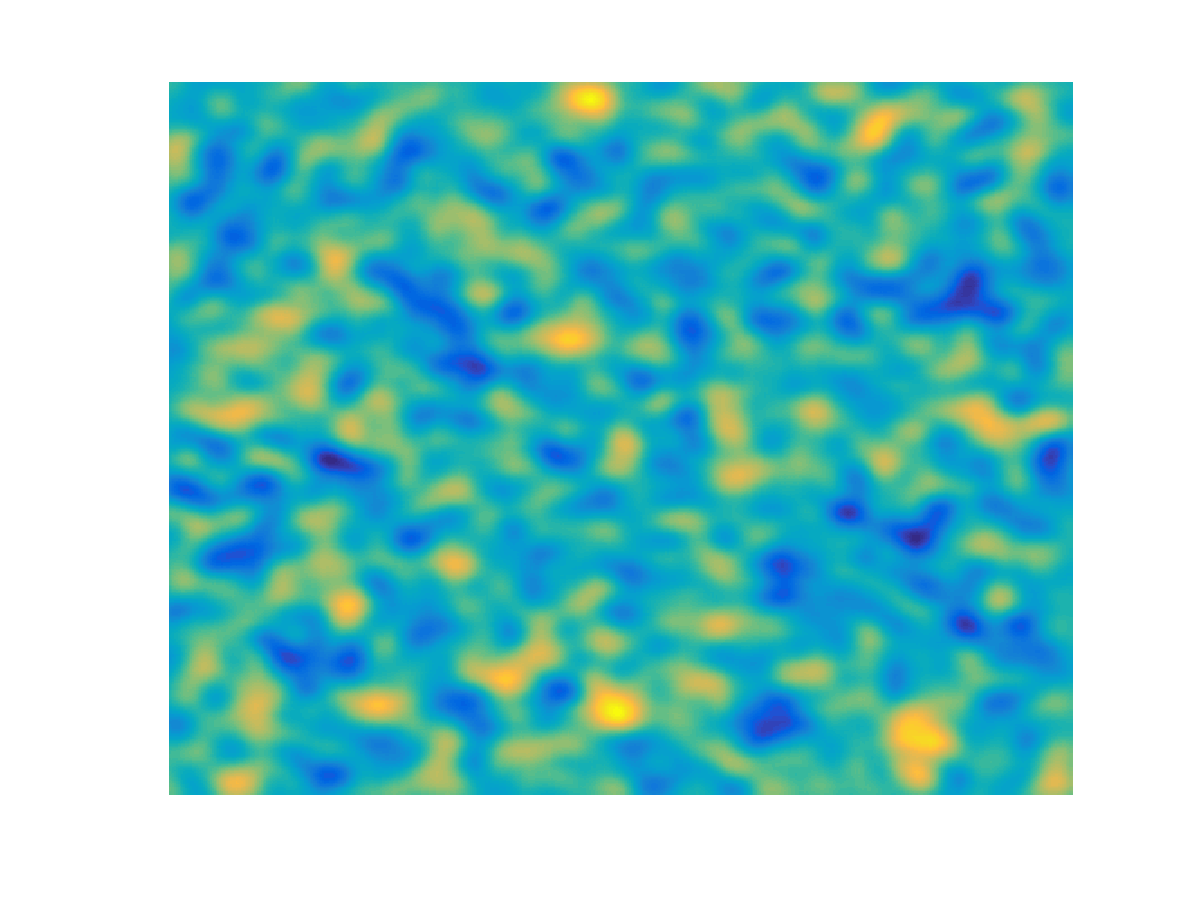
\includegraphics[width=0.49\linewidth]{random_field.eps} &
			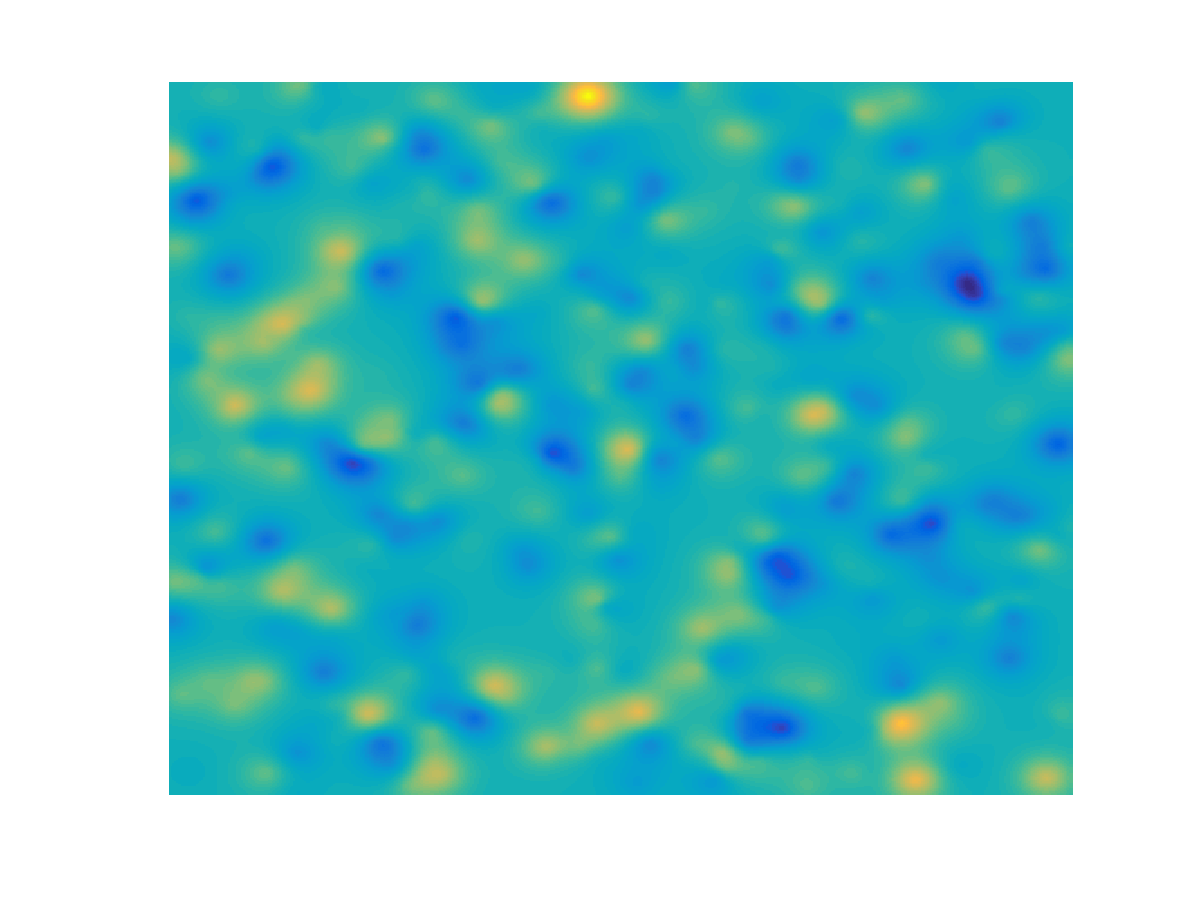
\includegraphics[width=0.49\linewidth]{kriging_prediction.eps} \\
			Randomly Generated Field & Kriging Method Predicted Field\\
		\end{tabular}
		\caption{A comparison of a random field generated using 500 random autocorrelated points, and a prediction of the field using the Kriging Method at randomly sampled points. \textit{figures generated using MATLAB.}}
	\end{figure}
\end{center}
The Kriging method also provides a variogram, with its prediction. The variogram provides a confidence score for each probability it computes via the computation of a discrete semi-variogram:\\
\begin{equation}
\hat{\gamma}({\bf{h}})=\dfrac{1}{2N({\bf{h}})}\sum_{i=1}^{N({\bf{h}})}\Big[Z(s_{i})-Z(s_{i}+{\bf{h}})\Big]^{2}
\end{equation}\\
Where $N({\bf{h}})$ is the number of pairs of data locations that are vector ${\bf{h}}$ apart.\\
The semi-variogram is then fit by a least squares to a continuous variogram that can be sampled for each point at question.
\begin{center}
	\begin{figure}[h]
		\centering
		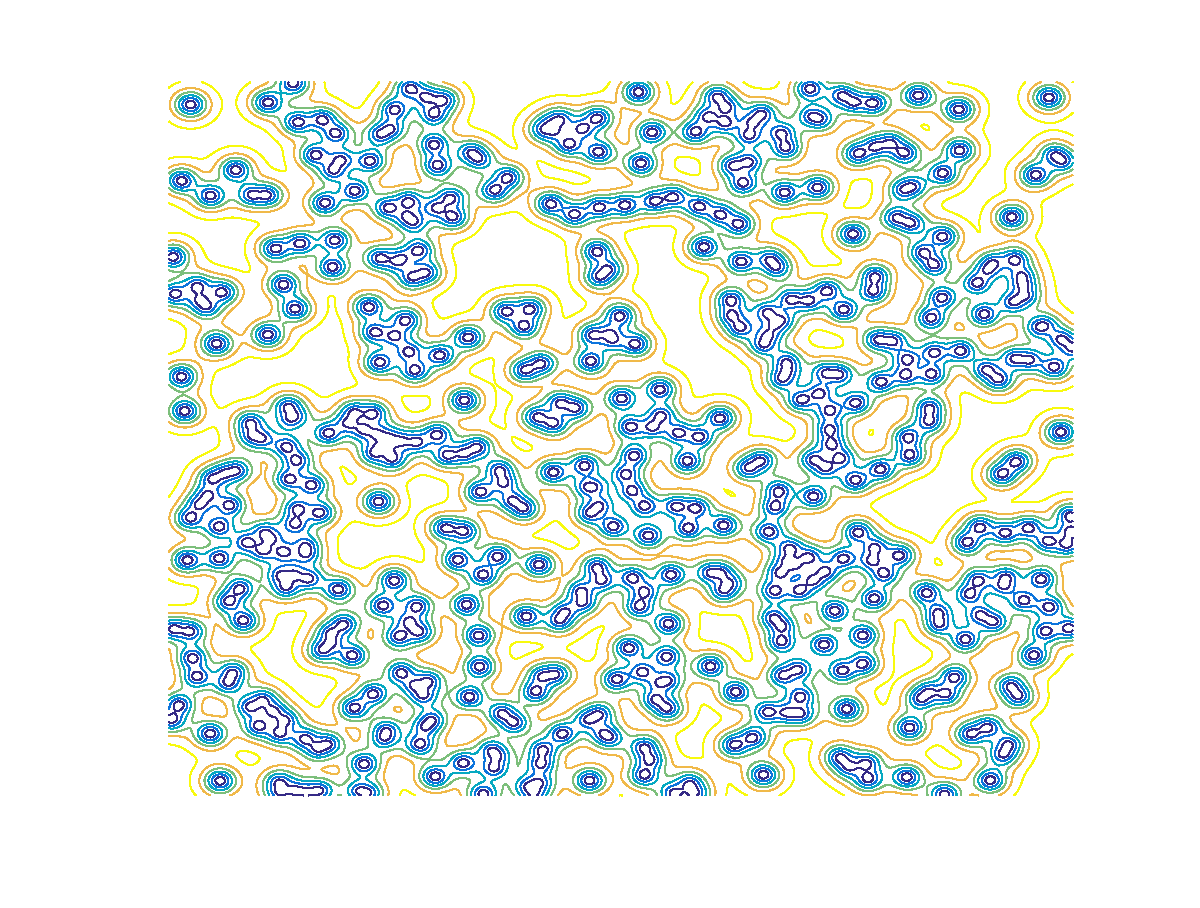
\includegraphics[scale=.5]{kriging_variance.eps}
		\caption{The variance of each prediction point from Figure 1. Larger spacing between the contours indicate greater variance. \textit{figure generated using MATLAB.}}
	\end{figure}
\end{center}
Although the method is optimal for data with no trends or drift, the use of the unmodified Kriging Method technique has the drawback of being computationally intensive and slow to compute in a live and timely manner. This is due to the multiple matrix inversions and least squares fittings to calculate the weights of the interpolation and the continuous variograms. It would be desired, in the case of autonomous UAVs that must constantly steer themselves in the best direction, to quickly calculate probabilities and covariances. \\
\subsection{Flying The Method}
\noindent
I began the development of a modified geostatistical interpolation method, based on the Kriging Method, to accomplish the task of fast and accurate autonomous UAV map scanning.\\
To decrease computation time, I will use Natural Neighbor Interpolation to calculate efficient areas of space to run the interpolation method on. This will remove the overhead of having to run a prediction on an entire area by reducing $N({\bf{h}})$ as much as possible without losing too much information from the interpolation, i.e. focus on individual chunks of the map one at a time. This modification reduces the dimensions of the matrices the regressions and predictions are being run on, dramatically reducing the time of the expensive computations.\\
\section{Goals}
\label{S:2}
\noindent
The method has proven to be a powerful interpolation method in simulations for simulated fields. The Kriging method has proven to be a working aerial mapping technique that provides a robust model for predictions and confidence scores. The goal of this thesis will be to design the algorithm for use with a pod of autonomous UAVs. A modified technique will have to first be developed to reduce the computational complexity of the algorithm by autonomously selecting optimal neighborhoods of sub-areas to run the method on.\\
Once the new method has been developed, an accurate simulation demonstrating its effectiveness and potential to be used in a real pod of UAVs will then be created and demonstrated. 
If time and resources are available, the algorithm will be ported to a real pod of UAVs to accomplish the task of autonomous scanning using thermal imaging (via infrared sensors). Tests will be conducted to prove the effectiveness and time efficiency of the newly developed algorithm.
%% The Appendices part is started with the command \appendix;
%% appendix sections are then done as normal sections
%% \appendix

%% \section{}
%% \label{}

%% References
%%
%% Following citation commands can be used in the body text:
%% Usage of \cite is as follows:
%%   \cite{key}          ==>>  [#]
%%   \cite[chap. 2]{key} ==>>  [#, chap. 2]
%%   \citet{key}         ==>>  Author [#]

%% References with bibTeX database:

\bibliographystyle{model1-num-names}
\bibliography{sample.bib}

%% Authors are advised to submit their bibtex database files. They are
%% requested to list a bibtex style file in the manuscript if they do
%% not want to use model1-num-names.bst.

%% References without bibTeX database:

% \begin{thebibliography}{00}

%% \bibitem must have the following form:
%%   \bibitem{key}...
%%

% \bibitem{}

% \end{thebibliography}


\end{document}

%%
%% End of file `elsarticle-template-1-num.tex'.